\documentclass[12pt,a4paper]{article}
\renewcommand{\baselinestretch}{1.05}
\usepackage[utf8]{inputenc}
\usepackage[spanish]{babel}


\usepackage{amsmath,amsthm,verbatim,amssymb,amsfonts,amscd, graphicx}
\usepackage{graphicx}
\usepackage{caption}
\usepackage{subcaption}
\usepackage{tkz-fct}
\usetikzlibrary{babel}
\usepackage{pgfplots}
\usepackage{booktabs}
\usepackage{float}
\usepackage{enumitem}
\usepackage{forest}
\usepackage{hyperref}
\usepackage{ragged2e}




\usepackage{xcolor}
\usepackage[tikz]{bclogo}
\usepackage[framemethod=tikz]{mdframed}
\usepackage{lipsum}
\usepackage[many]{tcolorbox}

\definecolor{bgblue}{RGB}{245,243,253}
\definecolor{ttblue}{RGB}{91,194,224}

\mdfdefinestyle{mystyle}{%
  rightline=true,
  innerleftmargin=10,
  innerrightmargin=10,
  outerlinewidth=3pt,
  topline=false,
  rightline=true,
  bottomline=false,
  skipabove=\topsep,
  skipbelow=\topsep
}

\newtcolorbox{myboxi}[1][]{
  breakable,
  title=#1,
  colback=white,
  colbacktitle=white,
  coltitle=black,
  fonttitle=\bfseries,
  bottomrule=0pt,
  toprule=0pt,
  leftrule=3pt,
  rightrule=3pt,
  titlerule=0pt,
  arc=0pt,
  outer arc=0pt,
  colframe=black,
}

\newtcolorbox{myboxii}[1][]{
  breakable,
  freelance,
  title=#1,
  colback=white,
  colbacktitle=white,
  coltitle=black,
  fonttitle=\bfseries,
  bottomrule=0pt,
  boxrule=0pt,
  colframe=white,
  overlay unbroken and first={
  \draw[red!75!black,line width=3pt]
    ([xshift=5pt]frame.north west) --
    (frame.north west) --
    (frame.south west);
  \draw[red!75!black,line width=3pt]
    ([xshift=-5pt]frame.north east) --
    (frame.north east) --
    (frame.south east);
  },
  overlay unbroken app={
  \draw[red!75!black,line width=3pt,line cap=rect]
    (frame.south west) --
    ([xshift=5pt]frame.south west);
  \draw[red!75!black,line width=3pt,line cap=rect]
    (frame.south east) --
    ([xshift=-5pt]frame.south east);
  },
  overlay middle and last={
  \draw[red!75!black,line width=3pt]
    (frame.north west) --
    (frame.south west);
  \draw[red!75!black,line width=3pt]
    (frame.north east) --
    (frame.south east);
  },
  overlay last app={
  \draw[red!75!black,line width=3pt,line cap=rect]
    (frame.south west) --
    ([xshift=5pt]frame.south west);
  \draw[red!75!black,line width=3pt,line cap=rect]
    (frame.south east) --
    ([xshift=-5pt]frame.south east);
  },
}





%Uso de la fuente Source Sans Pro

\usepackage[default]{sourcesanspro}
%\usepackage[T1]{fontenc}

%Controlar la partición de palabras.
\pretolerance=5000
\tolerance=6000

%Simbolo de euro
\usepackage{eurosym} % para el euro


%Definición de monospace para codigo inline y paquete listings para código fuente.
\def\code#1{\texttt{#1}}
\usepackage{listingsutf8}
\lstset{
    %extendedchars=false,
    %inputencoding=utf8
}
\usepackage{color}
\definecolor{grisclarito}{gray}{0.95}

\lstdefinestyle{customc}{
  %belowcaptionskip=1\baselineskip,
  breaklines=true,
  frame=single,
  %xleftmargin=\parindent,
  language=C,
  showstringspaces=false,
  %basicstyle=\ttfamily,
  keywordstyle=\bfseries\color{green!40!black},
  commentstyle=\itshape\color{purple!40!black},
  identifierstyle=\color{blue},
  stringstyle=\color{orange},
  backgroundcolor=\color{grisclarito}
}

\hypersetup{
  colorlinks=true,
  linkcolor=black,
  urlcolor=blue
}

\setlength{\parindent}{0pt}
\topmargin0.0cm
\headheight0.0cm
\headsep0.0cm
\oddsidemargin0.0cm
\textheight23.0cm
\textwidth16.5cm
\footskip1.0cm

\renewcommand*\contentsname{Índice}

\begin{document}
\pgfplotsset{compat=1.15}
\begin{titlepage}
  \centering
  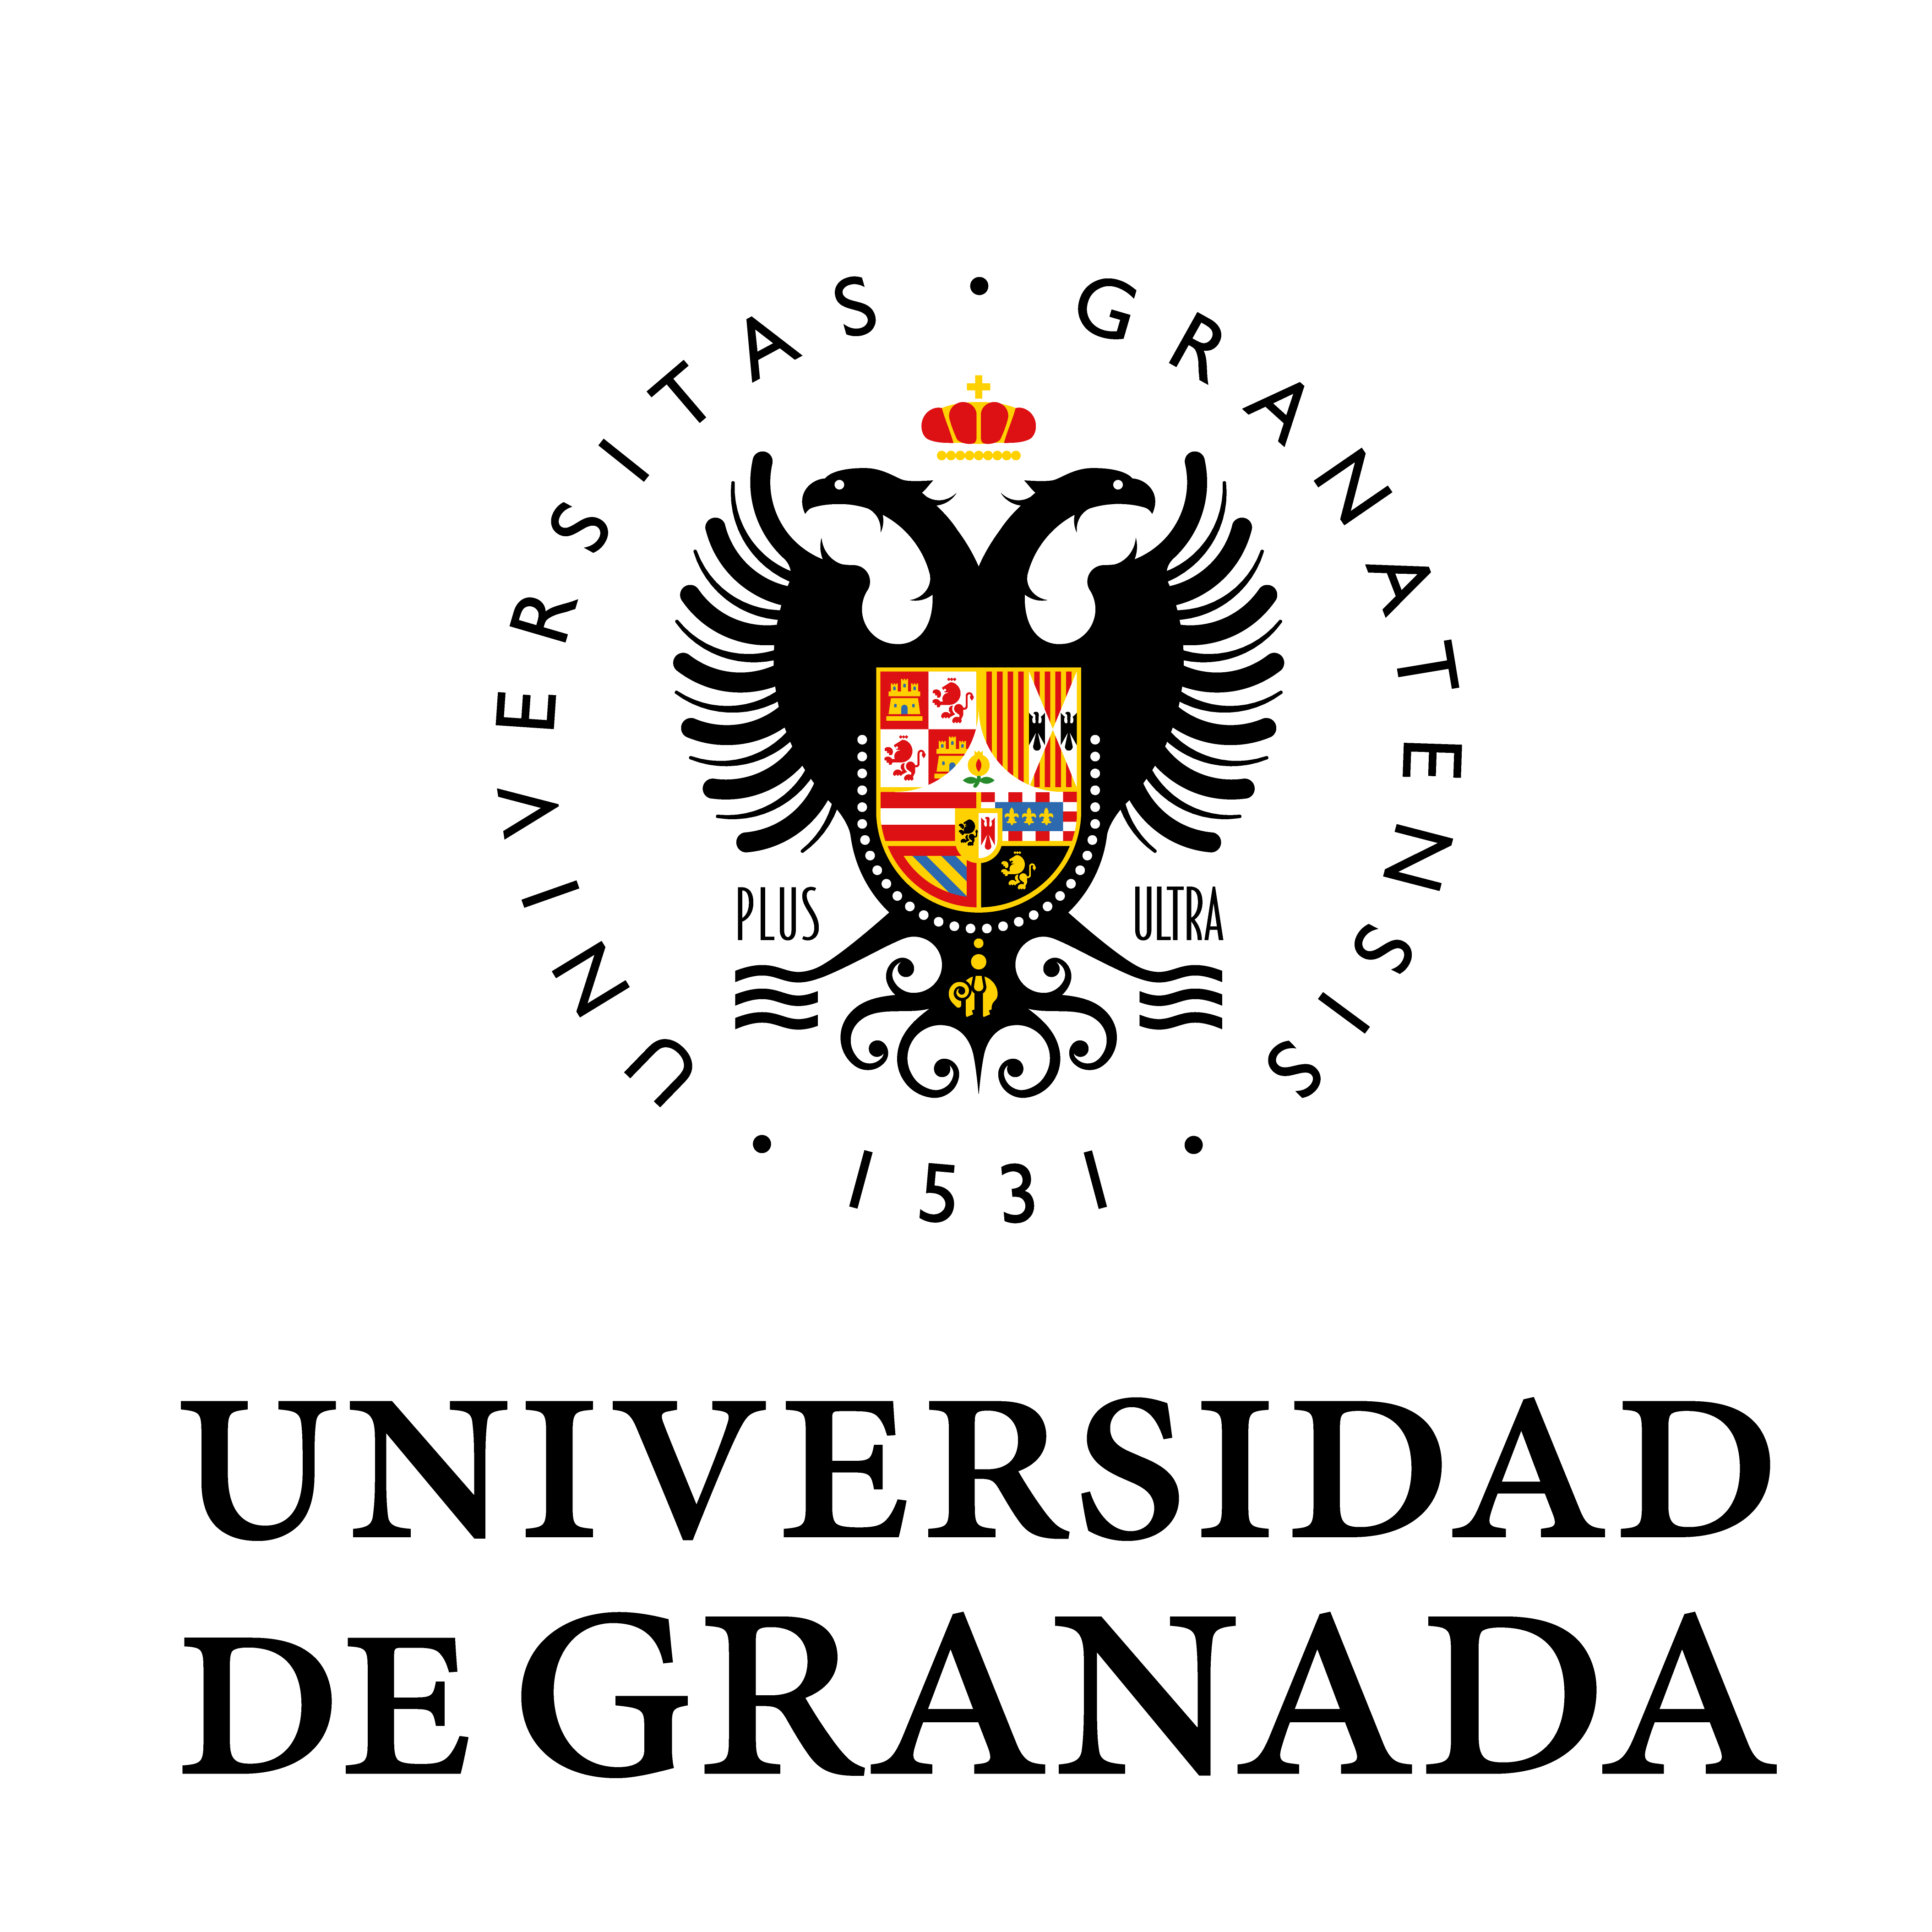
\includegraphics[width=0.6\textwidth]{ugr.png}\par\vspace{1cm}
  {\scshape\large Metodologías de desarrollo ágil \par} \vspace{1cm}
  {\huge\bfseries DSDM: Dynamic System Development Method \par}
  \vspace{0.4cm}
  {\large\itshape Un método iterativo y creciente\\}
  \vspace{0.6cm}
  {\large\itshape  Pedro Bonilla Nadal \\ David Infante Casas \\ Laura Gómez Garrido \\ Antonio Martín Ruiz \\ Juan Ocaña Valenzuela  \par} \vspace{1.00cm}
  Curso 2019-2020 \\
  \vfill

  % Bottom of the page
  {\large \today\par}
\end{titlepage}

\tableofcontents
\newpage

\setlength{\parskip}{10pt}

\section{Introducción}
El método de desarrollo de sistemas dinámicos (Dynamic Systems Development Method, DSDM) es un framework para el desarrollo de software de forma ágil creado en 1995 por lo que actualmente se conoce como el Consorcio DSDM. Esta metodología determina fases, subfases y principios que permiten a equipos de desarrollo trabajar de forma eficiente. Fue una metodología muy popular durante los años 90 y comparte cualidades con otros métodos de desarrollo ágil como SCRUM o Programación Extrema. Es por esto que no es una metodología muy explotada a día de hoy, pues muchos equipos prefieren el uso de SCRUM. DSDM se divide en tres fases: preproyecto, ciclo de vida del proyecto y postproyecto. A su vez, el ciclo de vida se subdivide en cuatro fases, viabilidad, exploración, ingeniería y despliegue.

\begin{center}
 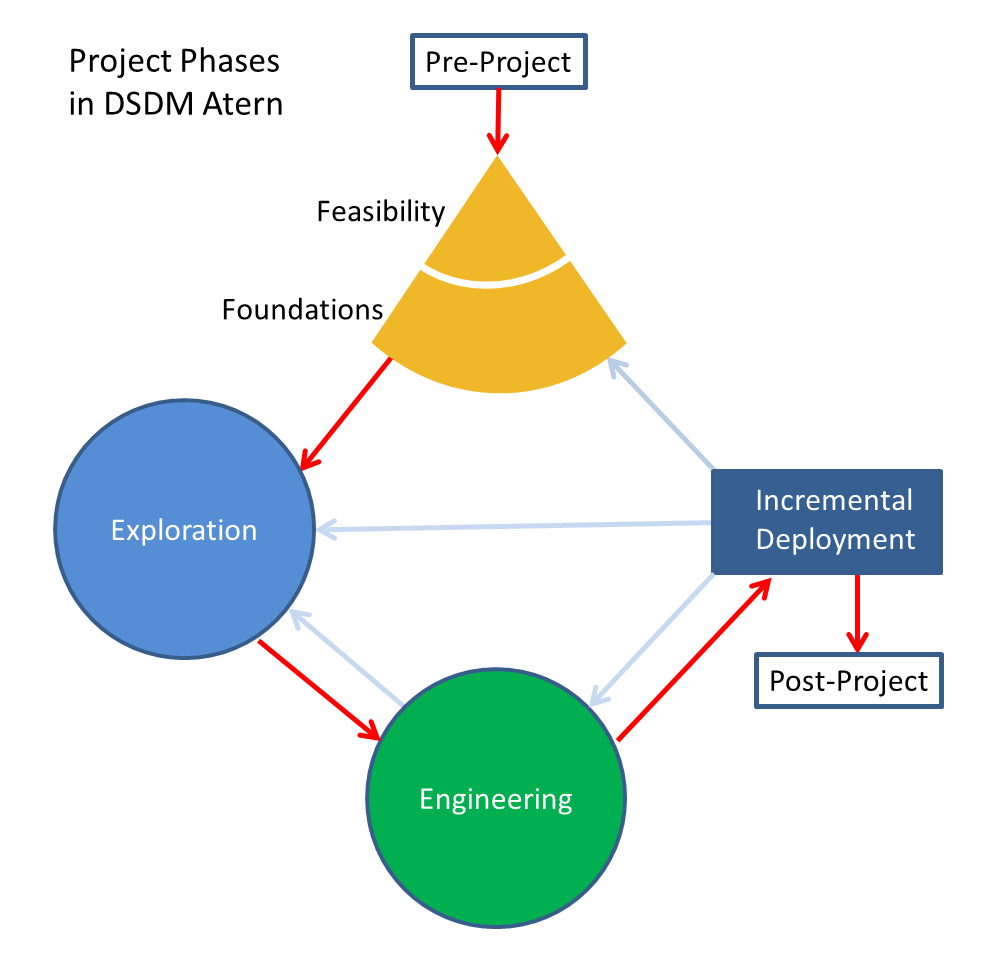
\includegraphics[width=0.6\textwidth]{DSDM_Phases.png}
\end{center}

DSDM es el método ágil más antiguo y es el único método ágil para centrarse en la gestión de proyectos ágiles. Arie van Bennekum representó a DSDM en el lanzamiento de Agile Alliance y su Agile Manifesto en 2001. DSDM opera principalmente en el ambiente corporativo donde demuestra consistentemente que es una métodología muy válida y permite completar exitosamente los procesos corporativos existentes. DSDM se ha ido actualizando a lo largo de los años, cuya última versión es Atern.


Algunas características de DSDM incluyen al usuario como componente activo durante el desarrollo, equipos bien preparados y lanzamiento de prototipos frecuente. También se usa la técnica <<Timeboxing>>, de la cual hablaremos más adelante, en la que se establecen intervalos en los que se liberarán los prototipos. Estos intervalos son muy similares a los sprints de SCRUM.



\section{Roles}
Entre los roles principales de la metodología DSDM, destacan:

\begin{itemize}
\item \underline{Patrocinador ejecutivo.} Es alguien que actúa como el CEO de una empresa. Ofrece recursos al proyecto y establece relaciones con el resto de ejecutivos relacionados al proyecto. También asegura la financiación del proyecto y una eficaz toma de decisiones.
\item \underline{Visionario.} Lo lleva a cabo alguien responsable de la detección inicial de requisitos para comenzar el proyecto, el cual también actúa como product manager. Motiva al equipo y les ofrece recursos de apoyo. Coordina los objetivos del proyecto con los de negocio.
También ayuda con el diseño y las sesiones de review.
\item \underline{Usuario embajador.} Es alguien con un gran conocimiento sobre el público objetivo y ofrece feedback al equipo de desarrollo. Se trata de un consultor externo. Comunica al equipo de desarrollo con el usuario. Trabaja en la detección de requisitos, diseño y sesiones de review. Ofrece visión de negocio para todas las decisiones que se toman. Ayuda al diseño y al testeo mostrando situaciones de negocio. Asegura que el producto final es el esperado.
\item \underline{Project manager.} Es responsable de que el proyecto se complete con éxito y el día a día del mismo. Realiza una planificación de alto nivel. Monitoriza el progreso, disponibilidad de recursos, configuración del proyecto, controla riesgos y problemas.
\item \underline{Desarrolladores.} Se encargan de la ingeniería y codificación del proyecto. No importa si el miembro del equipo es programador, analista o diseñador, todos se clasifican como desarrolladores.
\item \underline{Testers.} Su trabajo es probar y comprobar que el proyecto no contiene fallos y funciona correctamente. Define escenarios de prueba para el proyecto. Ofrece los datos de prueba obtenidos al líder del equipo.

\end{itemize}{}

\section{Fases del desarrollo}
Para explicar las fases de desarrollo, de entre las diversas variedades de DSDM, explicaremos en particular las del DSDM-Atern. Atern difiere de los enfoques ágiles más comunes en que abarca todo el ciclo de vida del proyecto y no sólo el desarrollo de software (donde prevalece SCRUM). Incorpora disciplinas de gestión de proyectos y proporciona mecanismos para asegurar que los beneficios del proyecto sean claros, que la solución propuesta sea factible y que existan bases sólidas antes de que se inicie el trabajo detallado.


\begin{itemize}
	\item \underline{Pre-proyecto}. Inicio del proyecto, acordando los Términos de Referencia para el trabajo. Es vital que durante esta fase el equipo satisfaga la mayoría de roles mencionados en su sección.
	\item \underline{Ciclo de vida del proyecto}. Está formado por las siguientes fases:
	\begin{itemize}
		\item \underline{Viabilidad}. Normalmente una fase corta en la que se realiza un estudio para asegurar cual es el valor del proyecto, coste y beneficio y resaltar su modelo de negocio.
		\item \underline{Fundaciones}. Fase clave para asegurar que el proyecto se entienda y defina lo suficientemente bien como para que el alcance se pueda basar en un alto nivel y los componentes y estándares tecnológicos se acuerden, antes de que comience la actividad de desarrollo. Durante esta fase se especifican los requisitos funcionales y no funcionales. Además los roles principales son Project Manager y CEO.
		\item \underline{Exploración}. Los líderes de proyecto y el equipo de desarrollo trabajan junto con el usuario embajador para asegurar un correcto desarrollo, detallando los requisitos previamente establecidos.
		\item \underline{Ingeniería}. Fase de desarrollo iterativo en la que la solución se diseña para que pueda desplegarse para su lanzamiento. El consultor externo se involucra para asegurar que las necesidades de los usuarios estén cubiertas.
		\item \underline{Despliegue}. Se presenta el sistema a los usuarios y se incorpora el feedback durante varias iteraciones.
	\end{itemize}
 	\item \underline{Post proyecto}. Evalúa los beneficios acumulados.
\end{itemize}

Las fases de exploración y la fase de ingeniería normalmente se mezclan, dado que el método es flexible, permite a los equipos que lo adapten trabajar dependiendo de la situación en la que se encuentren.


\section{Principios}
El método DSDM se usa para procesos de desarrollo ágil. Para mostrar como DSDM se relaciones es fundamental comprender los principio de DSDM y como estos se completan con las filosofías ágiles.\\

Los siguientes nueve principios son fundamentales para poder entender cual es la filosofía de desarrollo detrás de DSDM. En las descripciones de DSDM, si bien se explicita que no es necesario seguir al pie de la letra todas las fases del desarrollo, pues es un método adaptable a cada situación, si que explicitan que no seguir alguno de estos principios si que grava fuertemente el proceso de desarrollo.

\begin{enumerate}
	\item \underline{La participación activa del usuario}. Es imperativo este punto. Como bien sabemos uno de los principales aspectos de las metodologías ágiles es ser user-focused. El primer principio se considera el más importante, porque la participación de los usuarios a lo largo de todo el proyecto reduce efectivamente los errores en términos de percepción de los usuarios, y por lo tanto, reduce los costes de error. \\


En lugar de trabajar con un gran número de usuarios, las directrices de  DSDM  recomiendan trabajar con un pequeño y selecto grupo de usuarios continuamente, evitando así descubrir defectos solamente al final del proyecto en las reuniones con el usuario.\\


\item \underline{Los equipos deben tener poder para tomar decisiones}. Esto ayuda a proceder lo más rápidamente posible eliminando los costes de trasmisión y la espera de las comunicaciones. Estos retrasos y fricciones debido a la comunicación obligatoria entre equipo y gerentes deben ser evitadas. Solicitar
la autorización de recursos, incluso modestos, o cambios sencillos en los requisitos ralentizarán un proyecto de forma significativa.\\

 Del mismo modo los usuarios y otra gente involucrada en el proceso deben tener una autoridad, existente pero limitada para:
\begin{itemize}
	\item  Crear requisitos.
    \item Qué funcionalidad necesita estar en un incremento dado
    \item Priorización de requisitos y características
    \item Detalles de la solución técnica
\end{itemize}


\item \underline{Concentrarse en el lanzamiento y los límites de entrega.} Las entregas frecuentes de los resultados aseguran que los errores se detecten rápidamente, son fáciles subsanados y es más fácil de detectar la fuente del error. Esto se aplica tanto al código del programa como a la
así como a documentos como requisitos o modelos de datos.


\item \underline{Considerar como criterio para el software su validez en el mercado.}Como el nombre del marco de trabajo de DSDM sugiere, su esfuerzo principal es entregar
software que es lo suficientemente bueno para resolver la necesidad del negocio y preocuparse de cualquier mejora en una iteración posterior.


 DSDM no promueve la escritura ad-hoc sino que sugiere que se satisfagan  primero las necesidades del negocio, y que se usen TimeBoxes (explicadas posteriormente) para
refactorización y actividades relacionadas en una iteración posterior. Para ello es necesario que cosas como  la refactorización, ingeniería de diseño y mejora de características se consideren parte fundamental del proyecto. También es es crucial identificar en las primeras etapas del proyecto las cuestiones clave, que requieren un diseño robusto.




\item \underline{El desarrollo iterativo e incremental.}
Para reducir la complejidad del proyecto es necesario descomponerlo en pequeños paquetes de  características, y en cada iteración se añaden nuevas características hasta que todos los requisitos del negocio se cumplen.

 Este principio requiere aceptar el hecho de que que cualquier sistema de software está sujeto a cambios, uno de los principios universales de las metodologías ágiles. Este principio puede introducirse fácilmente incluso al principio de un proyecto, ya que las especificaciones y otros resultados pueden ser producido de manera iterativa también.


\item  \underline{Todos los cambios durante el desarrollo deben ser reversibles.} Para asegurar la capacidad de respuesta al cambio se requiere que las configuraciones del sistema cambien durante el desarrollo del proyecto debido a cambios en las prioridades de los requisitos.



\item \underline{Los requisitos se definen a alto nivel.} Para evitar limitar el grado de libertad con el que se pueden modificar los requisitos durante el proceso de desarrollo.  Estos requisitos se deben acordar durante el estudio de mercado del problema y después ser congelados.

\item  \underline{Las pruebas están integradas a lo largo de todo el ciclo de vida.} Muchos métodos de desarrollo, normalmente de carácter tradicional, requieren pruebas demasiado tarde como para que puedan tener un impacto poco costoso. DSDM requiere pruebas al principio del proceso de desarrollo.


\item \underline{Enfoque colaborativo y cooperativo.} Hay que evitar la separación y fomentar la colaboración entre el personal técnico y el personal empresarial
de un proyecto porque la cooperación es fundamental para llevar a cabo un proyecto de DSDM. Sin una atmósfera de confianza y honestidad será difícil obtener requisitos y un feedback conveniente.
\end{enumerate}

\section{Valores}

El Manifiesto Ágil desarrolla 4 principios fundamentales. En esta sección vamos a ver como DSDM se complementa con la filosofía ágil.

\begin{myboxii}[Recordatorio del Manifiesto Ágil]

Estamos descubriendo formas mejores de desarrollar software tanto por nuestra propia experiencia como ayudando a terceros. A través de este trabajo hemos aprendido a valorar:

    \begin{itemize}
    \item Individuos e interacciones sobre procesos y herramientas.
    \item Software funcionando sobre documentación extensiva.
    \item Colaboración con el cliente sobre negociación contractual.
    \item Respuesta ante el cambio sobre seguir un plan.
    \end{itemize}

Esto es, aunque valoramos los elementos de la derecha, valoramos más los de la izquierda.
\end{myboxii}

Analicemos uno a uno estos valores.

\subsection{Individuos}

Muchas metodologías de organización modernas expresan la importancia de considerar como individuos a los participantes del equipo. Los principios de DSDM 1 y 2 enfatizan este concepto, dando  a entender que tanto los integrantes del equipo son personas con capacidad de tomar decisiones de modo correcto y obligando una implicación de los usuarios activa, puesto que su opinión es importante.

De modo menos obvia, en los principios 3 y 5 también está escondido este concepto, al necesitar un ecosistema laboral sano para poder ser llevados a cabo.

\subsection{Software Funcionando}

El principio 4 recuerda que el éxito del software depende de su existo comercial, o al menos de su éxito de cara al usuario. Los principios 3 y 5 también hacen énfasis en este concepto al querer software funcionando de manera continua. Por último el principio 7 es fundamental para la comprensión de que es el Software Funcionando.


\subsection{Colaboración}

La colaboración es más significativa dado el principio 9 porque DSDM reacciona al cambio y cuando éste se produce, independientemente de que forme parte de un proyecto o de la vida personal, se requiere una buena cantidad de comunicación para resolver la implicación del cambio.  Poder hablar sin barreras  ayuda mucho. La necesidad de interpretar las declaraciones de otras personas y el error de malentendidos se reduce en gran medida.  Desafortunadamente, la colaboración no es fácil, ya que los humanos tienden a tomar decisiones egoístas, especialmente si se espera una recompensa inmediata.  La creación de un entorno en el que la colaboración funciona de la forma más fluida posible es una tarea de gestión y liderazgo.

\subsection{Respuesta al cambio}
Aceptar el cambio y responder a él tiene sus raíces en el principio 6 y parcialmente en el principio 7.  La gestión de las demandas cambiantes del negocio se percibe comúnmente como la diferencia más prominente de los métodos ágiles y tradicionales. DSDM maneja el cambio de varias maneras, principalmente a través de la priorización.

\section{TimeBoxing}
La gestión de proyectos tradicional utiliza \emph{miletones} para acordar un asset a realizar para un proyecto determinado en un determinado momento. Si bien los \emph{miletones} funcionan lo suficientemente bien, TimeBoxing es una técnica mucho más poderosa para lograr el mismo resultado. Una TimeBox es un intervalo, normalmente no más largo de 6 semanas, donde un conjunto dado de tareas debe ser logrado. El motivo de la duración relativamente baja de las TimeBox es el hecho de que los seres humanos dan estimaciones mucho más precisas en el futuro cercano, con un pequeño conjunto de tareas.
En las estimaciones de un futuro lejano, en el que intervienen grandes conjuntos de tareas, se acaban produciendo grandes errores.\\

 Una TimeBox puede contener varias tareas, y al final de esta se ha de entregar un producto. Los \emph{miletones} también
sufren de tener un entregable fijo, mientras que los TimeBoxes están sujetas a cambios, ya que se definen las tareas, no necesariamente el entregable, que puede cambiar si cambian las prioridades durante la iteración del TimeBox, lo que permite una respuesta rápida a necesidades del negocio. En resumen, DSDM deja de lado la funcionalidad a favor de la entregar a tiempo.

Podemos observar como características en el uso de timeboxing en combinación con las fases del proyecto DSDM:
\begin{enumerate}
	\item  Los Timeboxes pueden ser de diferente longitud.
	\item  Varias de las mismas fases de DSDM pueden ejecutarse inmediatamente después de la TimeBox de la misma fase si ha terminado.
\item Las TimeBoxes paralelas son posibles, incluso las TimeBoxes complementarias son permitidas.
\item Diferentes fases de DSDM pueden ser realizadas en una TimeBox al mismo tiempo.
\item Las Timeboxes pueden ser anidadas.
\end{enumerate}


{\color{red} \rule{\linewidth}{0.5mm} }
{\color{blue} TODO: hola, podemos añadir de la página https://www.methodsandtools.com/archive/dsdmatern.php cuales son los princpipiso, los roles y los productos.}\\
{\color{red} \rule{\linewidth}{0.5mm} }

%Bibliographic references
\begin{thebibliography}{9}

\bibitem{pickpocketing} Dynamic Systems Development Method (DSDM)
\\\texttt{http://www.students.science.uu.nl/~slegt001/me/final\_5767202\_Slegten.pdf}
\bibitem{pickpocketing2}Dynamic System Development Method
\\\texttt{https://files.ifi.uzh.ch/rerg/arvo/courses/seminar\_ws03/14\_Voigt\_DSMD\_Ausa-\\rbeitung.pdf}
\bibitem{pickpocketing3}New Directions on Agile Methods:A Comparative Analysis
\\\texttt{http://secure.com.sg/courses/ICT353/Session\_Collateral/TOP\_03\_ART\_06\_ARTI-\\CLE\_ABRAHAMSSON\_New\_Directions\_Agile\_Methods.pdf}

\bibitem{pickpocketing4}Agile software developmentmethods.
\\\texttt{http://www.vtt.fi/inf/pdf/publications/2002/P478.pdf}


\bibitem{pickpocketing5}Introduction to DSDM Atern
\\\texttt{https://www.methodsandtools.com/archive/dsdmatern.php}
\end{thebibliography}

\end{document}
